\documentclass{article}
\usepackage{hyperref}
\usepackage{graphicx}
\usepackage{listings}
\usepackage{caption}

\lstset{
  breaklines=true, 
  breakatwhitespace=true, 
  basicstyle=\small\ttfamily, 
  columns=fullflexible 
}

\title{Using Large Language Models for structured information extraction from the IPNO case files}

\author{
    Ayyub Ibrahim\footnote{\href{https://ip-no.org/who-we-are/staff/}{Ayyub Ibrahim's Profile}} \\
    Director of Research for LLEAD, IPNO
    \and
    Tarak Shah\footnote{\href{https://hrdag.org/people/tarak-shah/}{Tarak Shah's Profile}} \\
    Data Scientist, HRDAG
}

\begin{document}
\maketitle

\section*{Abstract}
Exoneration documents, secured during legal proceedings that aim to right the wrongs of justice, are invaluable for understanding wrongful convictions. They cast a spotlight on law enforcement actions, revealing systemic challenges. Yet, finding and leveraging usable information within these collections remains a formidable task for researchers and advocates, due to their volume and unstructured heterogeneity. This paper introduces the methodology of the Innocence Discovery Lab—a collaboration between Innocence Project New Orleans (IPNO) and the Human Rights Data Analysis Group (HRDAG). By developing a comprehensive index for these documents, targeting specific files, and analyzing cross-referenced data, we aim to unearth patterns and systemic issues that underpin wrongful convictions.

\section{Introduction}

In October 2022, IPNO launched \href{https://llead.co/}{Law Enforcement Accountability Database (LLEAD)}, a consolidation of data from over 500 law enforcement agencies in Louisiana. To date, LLEAD hosts details of over 40,000 allegations of misconduct spanning 194 agencies across 48 of Louisiana's 64 parishes. This initiative is the first state-wide database of its kind. LLEAD is already an essential tool for exoneration work, and including wrongful conviction information in the database would make it even more useful. For example, in Orleans Parish, Louisiana, 78\% of wrongful convictions have been linked to law enforcement's failure to share exculpatory evidence with the defense, a rate more than double the national average. Given this backdrop, we seek to make these collections searchable and useful for lawyers, advocates, and community members to better investigate patterns of police misconduct and corruption. In order to do so, we rely on a multi-stage process:

\begin{enumerate}
    \item Metadata Compilation:
    \begin{itemize}
        \item file path and name
        \item file type
        \item sha1 content hash: we truncate this to create unique file identifiers
        \item file size and number of pages
        \item case ID: when we scanned the documents, we organized them into directories organized by case ID, here we pluck and validate the directory name to add a structured case id field to our metadata index.
    \end{itemize}
    
    \item Page classification:
    \begin{itemize}
        \item police reports: include mentions of officers involved in the arrest that led to the wrongful conviction, or related arrests.
        \item transcripts: court transcripts, recorded by clerks of the court, where officers appear as witnesses and describe their role in the conviction (including making the arrest, transporting evidence, interrogating the accused).
        \item testimonies: witness testimony, which will include testimony from officers involved in the conviction        
        \item page classification: page classification involves building a classification model to categorize files (or page sequences within files) into these different types of documents. One approach is to fine-tune a pretrained convolutional neural network to label thumbnail images of document pages. Using thumbnails is advantageous because they are smaller files, resulting in faster processing and reduced computational resource consumption. This makes them an effective approach for retrieving specific types of documents from disorganized collections, as described in \href{https://arxiv.org/abs/1502.07058}{Evaluation of Deep Convolutional Nets for Document Image Classification and Retrieval}. In order to use this technique, we needed training data and a pretrained model. To quickly assemble a training data set for our page classifier, we started by noticing that in many cases the file name indicated the document type. These documents were scanned by many people at different times, so we could not rely on this heuristic for comprehensive categorization of documents, but there was more than enough there to jumpstart our training process. We collected our initial training data by probing filenames for specific search terms, and reviewing and confirming that we had inferred the correct document types from the filenames. Once we had training data, we used [FastAI](https://docs.fast.ai/) to fine-tune the `ResNet34` architecture, pretrained on [ImageNet](https://www.image-net.org/), to identify reports, transcripts, and testimonies based on page thumbnails. With the trained classifier, we were able to measure generalization performance on documents that couldn't be classified via filename, and we were also better able to target additional training data, for example by reviewing pages where the classifier had low confidence about its prediction. 
    \end{itemize}
    
    \item Information Extraction: Currently, we're engaged in extracting structured information from the documents we've identified, and that work is the focus of the current post. Our goal is to extract structured information related to each police officer or prosecutor mentioned in the documents, such as their names, ranks, and roles in the wrongful conviction.

    \item Deduplication: The previous step leaves us with many distinct mentions, but some individuals are mentioned many times, within the same case or across cases. Here we rely on HRDAG's \href{https://hrdag.org/tech-notes/adaptive-blocking-writeup-1.html}{extensive experience with database deduplication} to create a unique index of officers and prosecutors involved in wrongful convictions, and a record and the role or roles they had in the wrongful conviction.

    \item Cross-referencing: In the final stage, we'll cross-reference the officer names and roles we've extracted with the Louisiana Law Enforcement Accountability Database \href{https://llead.co/}{(LLEAD)} to identify other cases these officers have been involved in.
\end{enumerate}

A primary task in our process is extracting officer information from documents – specifically, the officer's name and the role the officer played in the wrongful conviction. The extraction of such information is crucial for understanding the dynamics and potential lapses that led to the conviction. Given the importance of this task, it's essential to approach it with a methodology that ensures accuracy and comprehensiveness.

We initially considered a regex-based solution for this extraction task. Regular expressions, or regexes, are powerful tools for pattern matching within text. However, as we delved deeper into our data, we realized that the complexity and variability of the content rendered regex less than ideal. While regex excels at identifying specific patterns within text, it often struggles with variations in language and nuances that commonly appear in natural language texts, such as police reports and court transcripts.

Consider the text string from a court transcript reading, "Sergeant Ruiz was mentioned as being involved in the joint investigation with Detective Martin Venezia regarding the Seafood City burglary and the murder of Kathy Ulfers." Such a sentence poses challenges for regex due to its inability to capture semantic context. Without understanding the broader narrative, regex cannot infer that Sergeant Ruiz acted as a lead detective in Kathy Ulfers' murder case.

To further highlight the limitations of regex in handling such tasks, we designed a simple baseline model. Instead of attempting to capture the full scope of officer information extraction, this model focuses solely on extracting officer names as a starting point. This choice was intentional; by narrowing down the task, we hoped to provide a clear example of the strengths and weaknesses of regex in the context of real-world data.

\begin{lstlisting}[language=Python, caption=Code Snippet 1]
    pattern = re.compile(
        r"(detective|sergeant|lieutenant|captain|corporal|deputy|"
        r"criminalist|technician|investigator|det\.|sgt\.|lt\.|cpt\.|"
        r"cpl\.|dty\.|tech\.|dr\.)"
        r"\s+([A-Z][A-Za-z]*(\s[A-Z][A-Za-z]*)?)", 
        re.IGNORECASE
    )
\end{lstlisting}

\begin{itemize}
    \item After implementing our baseline model, we tested its performance on two different sets of data: police reports and court transcripts.
    \item \textbf{Police Reports Results:}
    \item \textbf{Precision}: 0.845: This indicates that among the instances our model predicted as officer names, 84.5\% of them were indeed officer names. A high precision suggests that the model is quite reliable in its positive predictions.
    \item \textbf{Recall}: 0.518: This metric reveals that our model was able to identify only 51.8\% of the actual officer names present in the police reports. A lower recall signifies that while our predictions are accurate, we are missing out on a significant number of true officer names.
    \item \textbf{F1 Score}: 0.614: The F1 score harmonizes precision and recall, giving us a balanced view of the model's performance. At 0.614, it suggests that there is room for improvement, especially in capturing more true positives without sacrificing precision.
    \item \textbf{F\_beta}: 0.549: This score is another harmonic mean of precision and recall but gives more weight to recall. A score of 0.549 further emphasizes the model's challenges in identifying all true positives.
    \item \textbf{Court Transcripts Results:}
    \item \textbf{Precision}: 0.8656: Similar to the police reports, our model displayed high precision on court transcripts, indicating its reliability in positive predictions.
    \item \textbf{Recall}: 0.4281: However, the recall is notably lower on the court transcripts, meaning our model missed out on more than half of the actual officer names present in these documents.
    \item \textbf{F1 Score}: 0.5461: The F1 score for court transcripts is lower than that for police reports, suggesting a more pronounced trade-off between precision and recall in this dataset.
    \item \textbf{F\_beta}: 0.4663: Once again, the F\_beta score underscores the need for improving recall without compromising precision.
\end{itemize}

While our regex-based baseline model exhibits high precision on both datasets, it struggles notably with recall. This indicates that while the names it identifies as officers are likely correct, it misses a substantial number of actual officer names present in the documents. These findings further emphasize the challenges of using regex alone for such a complex task and underscore the need for more advanced techniques that can capture the nuances and variations in language.

An alternative approach is to prompt a generative language model with the document text along with a query describing our required output. One challenge with this approach is that the documents we're processing may be hundreds of pages long, whereas generative models have a limit to the length of the prompt you supply. We needed a way to pull out of each document just the chunks of text where the relevant officer information appears, to provide a more helpful prompt.

We split up the problem into two steps, identifying the relevant chunks of text content, and then extracting structured officer information from those chunks. We use \href{https://docs.langchain.com/docs/}{Langchain}, a natural language processing library, to manage this pipeline, and use OpenAI's language model, GPT-3-Turbo-16k as the language model powering the pipeline.

For the first step, identifying the relevant chunks of text within the larger document, we used the approach outlined in \href{https://arxiv.org/abs/2212.10496}{Precise Zero-Shot Dense Retrieval without Relevance Labels}. This approach splits our information retrieval task into multiple steps:

\begin{enumerate}
    \item We feed our query asking for names and roles of mentioned officers to an instruction-following generative language model, instructing it to compose a "hypothetical" document in response to the query.
    \item We embed the hypothetical document.
    \item We chunk the document text into overlapping chunks, and calculate embeddings for each chunk using the same embedding system we used for the hypothetical document.
    \item We use \href{https://faiss.ai/}{Faiss} to do similarity search, using similarity to our hypothetical document embeddings to identify chunks of relevant text content.
\end{enumerate}

Here is the method we use to generate hypothetical embeddings. The resulting object can be used to embed chunks of text, enabling efficient similarity search over them.

\begin{lstlisting}[language=Python, caption=Code Snippet 2, breaklines=true]
    PROMPT_TEMPLATE_HYDE = PromptTemplate(
        input_variables=["question"],
        template="""
        You're an AI assistant specializing in criminal justice research. 
        
        Your main focus is on identifying the names and providing detailed context of mention for each law enforcement personnel. 
        
        This includes police officers, detectives, deputies, lieutenants, sergeants, captains, technicians, coroners, investigators, patrolmen, and criminalists, as described in court transcripts and police reports.

        Question: {question}
        Roles and Responses:"""
    )
\end{lstlisting}

\begin{lstlisting}[language=Python, caption=Code Snippet 3, breaklines=true]
    def generate_hypothetical_embeddings():
        llm = OpenAI()
        prompt = PROMPT_TEMPLATE_HYDE
        llm_chain = LLMChain(llm=llm, prompt=prompt)
        base_embeddings = OpenAIEmbeddings()
        embeddings = HypotheticalDocumentEmbedder(
            llm_chain=llm_chain, base_embeddings=base_embeddings
        )
        return embeddings
\end{lstlisting}

The \texttt{process\_single\_document} function converts an input document into a vector database of chunks. This function employs Langchain's RecursiveCharacterTextSplitter to split documents into chunks of 500 tokens, while maintaining an overlap of 250 tokens to ensure contextual continuity.

There are times when the model might inadvertently identify names without clear ties to law enforcement personnel. By cross-referencing the model's output with LLEAD, we believe we will be able to filter out many such false positives (it's worth noting that some law enforcement personnel mentioned in the documents will be absent from LLEAD, but our current focus is on officers we can track using LLEAD). On the other hand, we have no way of recovering officer mentions if they are not picked up by our extraction process. In light of this, when evaluating the model we are more interested in maximizing recall, ensuring we identify as many genuine law enforcement mentions as we can.  To quantify this focus on recall, we employed the \href{https://en.wikipedia.org/wiki/F-score#F%CE%B2\_score}{F-beta score} (with $\beta=2$), which weighs recall twice as heavily as precision. We tested the model using varying chunk sizes, including 2000, 1000, and 500, with corresponding overlaps of 1000, 500, and 250 respectively. Based on our evaluations, the optimal configuration is a chunk size of 500 with an overlap of 250. After segmentation, the text is transformed into a high-dimensional space using precomputed embeddings from our hypothetical document embedder. The \texttt{FAISS.from\_documents} function aids in this transformation, constructing an indexed document database designed for similarity searches.

\begin{lstlisting}[language=Python, caption=Code Snippet 4, breaklines=true]
    def process_single_document(file_path, embeddings):
        logger.info(f"Processing document: {file_path}")
        loader = JSONLoader(file_path)
        text = loader.load()
        logger.info(f"Text loaded from document: {file_path}")
        text_splitter = RecursiveCharacterTextSplitter(chunk_size=500, chunk_overlap=250)
        docs = text_splitter.split_documents(text)
        db = FAISS.from_documents(docs, embeddings)
        return db
\end{lstlisting}

In the following sections, we define the core function \texttt{get\_response\_from\_query(db, query)}. This function serves as the backbone of our information extraction process, taking in a document database and a query, and returning the system's response to the query. 

The process begins by setting up the relevant parameters. We use a prompt template to guide the query and a role template to define the roles we're interested in. We set the temperature parameter to 0 to maximize the determinism of our responses. The k parameter is set to 20, a decision guided by the F-beta score results from our testing phase, instructing the system to select and concatenate the top 20 relevant text chunks from the document corpus. These documents are then sorted by similarity score to maximize the model's performance. As suggested in the paper \href{https://arxiv.org/abs/2307.03172}{Lost in the Middle: How Language Models Use Long Contexts}, for retrieval tasks current language models perform best when the relevant data is located at the beginning of their context window.

The relevant chunks of text are then passed to the \texttt{LLMChain} class of the LangChain module as part of the 'run' method. In addition to relevant chunks, the 'run' method also receives the \texttt{PromptTemplate}, \texttt{RoleTemplate}, and the original query.

The \texttt{LLMChain} processes these inputs and generates a structured response to the initial query.

\begin{lstlisting}[language={}, breaklines=true, caption=Code Snippet 5]
    PROMPT_TEMPLATE_MODEL = PromptTemplate(
        input_variables=["roles", "question", "docs"],
        template="""
        As an AI assistant, my role is to meticulously analyze court transcripts, traditional officer roles, and extract information about law enforcement personnel.
    
        Query: {question}
    
        Transcripts: {docs}
    
        Roles: {roles}
    
        The response will contain:
    
        1 The name of an officer, detective, deputy, lieutenant, sergeant, captain, officer, coroner, investigator, criminalist, patrolman, or technician - if an individual's name is not associated with one of these titles they do not work in law enforcement. Please prefix the name with "Officer Name: ". For example, "Officer Name: John Smith".
    
        2 If available, provide an in-depth description of the context of their mention. If the context induces ambiguity regarding the individual's employment in law enforcement, remove the individual. Please prefix this information with "Officer Context: ". 
    
        3 Review the context to discern the role of the officer. Please prefix this information with "Officer Role: ". For example, the column "Officer Role: Lead Detective" will be filled with a value of 1 for officers who were the lead detective.
    """,
    
    ROLE_TEMPLATE = """
    US-IPNO-Exonerations: Model Evaluation Guide 
    Roles:
    Lead Detective
    1. Coordinates with other detectives and law enforcement officers on the case.
    2. Liaises with the prosecutor's office, contributing to legal strategy and court proceedings.

    Crime Lab Analyst
    1. Analyses various types of evidence gathered during an investigation, including but not limited to, DNA, fingerprints, blood samples, drug substances, etc.
    2. Prepares detailed reports outlining the findings of their analyses.
    """
\end{lstlisting}

\begin{lstlisting}[language=Python, caption=Code Snippet 6, breaklines=true]
    def get_response_from_query(db, query):
        # Set up the parameters
        prompt = PROMPT_TEMPLATE_MODEL
        roles = ROLE_TEMPLATE
        temperature = 0
        k = 20
    
        # Perform the similarity search
        doc_list = db.similarity_search_with_score(query, k=k)

        # sort documents by relevance score 
        docs = sorted(doc_list, key=lambda x: x[1], reverse=True)
        
        third = len(docs) // 3
        highest_third = docs[:third]
        middle_third = docs[third:2*third]
        lowest_third = docs[2*third:]
        highest_third = sorted(highest_third, key=lambda x: x[1], reverse=True)
        middle_third = sorted(middle_third, key=lambda x: x[1], reverse=True)
        lowest_third = sorted(lowest_third, key=lambda x: x[1], reverse=True)
    
        docs = highest_third + lowest_third + middle_third

        # concatenate documents
        docs_page_content = " ".join([d[0].page_content for d in docs])
    
        # Create an instance of the OpenAI model
        llm = ChatOpenAI(model_name="gpt-3.5-turbo")
    
        # Create an instance of the LLMChain
        chain = LLMChain(llm=llm, prompt=prompt)
    
        # Run the LLMChain and print the response
        response = chain.run(roles=roles, 
                             question=query, 
                             docs=docs_page_content, 
                             temperature=temperature)
        return response
\end{lstlisting}

\subsection{Model Contextual Inputs and Outputs}

For additional context, the following showcases the inputs and outputs of our approach:

\vspace{1em} 

\noindent \textbf{Query}:``Identify individuals, by name, with the specific titles of officers, sergeants, lieutenants, captains, detectives, homicide officers, and crime lab personnel in the transcript. Specifically, provide the context of their mention related to key events in the case, if available."

\vspace{1em} 

\noindent \textbf{Relevant Document}:  
(1 of 20 documents identified by the Faiss similarity search as relevant)

\begin{quote}
Martin Venezia, New Orleans police sergeant.\\
``A 16 .01 Sergeant Venezia, where are you assigned now?"\\
``A Second Police District. 13 . And in October, September of 1979 and in Q 19 September and October of 1980, where were you assigned? :1 Homicide division. A. And how long have you been on the police department right now? Thirteen and a half years. A Officer Venezia, when did you or did you ever take over the investigation of ... Cathy Ulfers' murder? A"
\end{quote}

\vspace{1em} 

\textit{metadata}: \{'source': '../../data/convictions/transcripts/iterative(C) Det. Martin Venezia Testimony Trial One.docx'\}

\vspace{1em}

\noindent \textbf{Response from the Model}:

\begin{itemize}
    \item \textbf{Officer Name}: Sergeant Martin Venezia  
    \item \textbf{Officer Context}: Sergeant Martin Venezia, formerly assigned to the Homicide Division, took over the investigation of Cathy Ulfers' murder.  
    \item \textbf{Officer Role}: Lead Detective
\end{itemize}

\section{Evaluations, issues, improvements}

In our effort to optimize the model's capability to extract officer names from documents, we evaluated it on various parameters. The following tests were run using GPT-4.

\noindent \textbf{Preprocessing Parameters}:
\begin{itemize}
    \item \textbf{Chunk Size}: Defines the number of consecutive words or units of text processed at once.
    \item \textbf{Chunk Overlap}: This parameter dictates the number of words consecutive chunks share. For example, with an overlap of 250, the subsequent chunk begins 250 words into the previous chunk.
\end{itemize}

\noindent \textbf{Model-specific Parameters}:
\begin{itemize}
    \item \textbf{Hypothetical Document Embeddings (HYDE)}: Investigated their effect on the model's overall performance.
    \item \textbf{'k' Value}: Denotes the number of text chunks input to the model.
    \item \textbf{Temperature Parameter}: Influences the randomness of the model.
\end{itemize}

For evaluating our model's performance, we utilized the F-beta score as our primary metric. Unlike the F1 score, which gives equal weight to precision (correctness) and recall (completeness), the F-beta score allows for differential weighting. We designed our score to weigh recall twice as much as precision, reflecting the importance of accurately spotting relevant information, even if it means occasionally flagging some irrelevant content.

Based on our evaluations, our model performed best with:
\begin{itemize}
    \item Chunk size of 500
    \item Chunk overlap of 250
    \item Integration of HYDE embeddings
    \item 'k' value of 20
\end{itemize}

For police reports, the F-beta score reached 0.864909, while for transcripts, the F-beta score peaked at 0.813397.

Although larger chunk sizes, such as 1000 and 2000, might offer advantages for certain applications, they resulted in lower F-beta scores during our tests. Similarly, greater overlaps like 500 and 1000 reduced our performance, even with the potential for more context. The consistent advantage of incorporating HYDE embeddings was evident, underscoring their value to our model.

Another key observation was regarding the temperature parameter, which influences the model's level of randomness. With a temperature set to 1, we generally saw higher F-beta scores, especially for identifying officer names in police reports. As we move to the next phase — extracting detailed context about the officers role within the document — the precise handling of this parameter will be crucial because a high temperature can potentially skew results or generate "hallucinated" content.

\subsection{Model Behavior Analysis Over Iterative Runs}

After our evaluation of the model based on various parameters, the next phase delved into understanding the model's behavior over iterative runs. Due to the stochastic nature of generative text models, a single document can yield diverse outputs when processed multiple times using the same parameters. This highlighted the challenge of identifying an optimal number of iterations, a balance that ensures comprehensive insights while being cost efficient. In the interest of cost efficiency, the following tests were run using GPT-3.5-Turbo-16K. The decline in performance can be attributed to the change in model. 

To address this, we employed two distinct query strategies:

\subsubsection{Multiple Queries Approach}

This strategy used six unique queries, each crafted to extract specific facets of the required information. The queries are as follows:

\begin{enumerate}
    \item \textbf{Query 1:} Identify individuals, by name, with specific titles mentioned. Provide context related to key events in the case.
    \item \textbf{Query 2:} List individuals and detail the significant decisions or actions they undertook.
    \item \textbf{Query 3:} Locate individuals and discuss their interactions with other case individuals.
    \item \textbf{Query 4:} Highlight individuals and describe their roles or responsibilities.
    \item \textbf{Query 5:} Outline individuals and specify any noteworthy outcomes they achieved.
    \item \textbf{Query 6:} Pinpoint individuals and emphasize significant incidents they were part of.
\end{enumerate}

\subsubsection{Singular Query Approach}

This method employed a comprehensive query, designed to holistically capture all the desired information facets. We run the document through the same query repeatedly, which results in slightly different responses each time, and then collect the results together. The query is:

\begin{quote}
\textbf{Query:} Identify each individual and present a contextual description that includes their decisions, interactions, roles, outcomes, and any significant incidents.
\end{quote}

In the context of police reports, a detailed analysis of the singular query method showed that its performance metrics improved with each iteration up to the 4th iteration, with a marked increase in the F1 Beta score after each iteration. However, past this iteration, the incremental gains in the score reduced, indicating we had hit the point of diminishing returns.

\begin{center}
    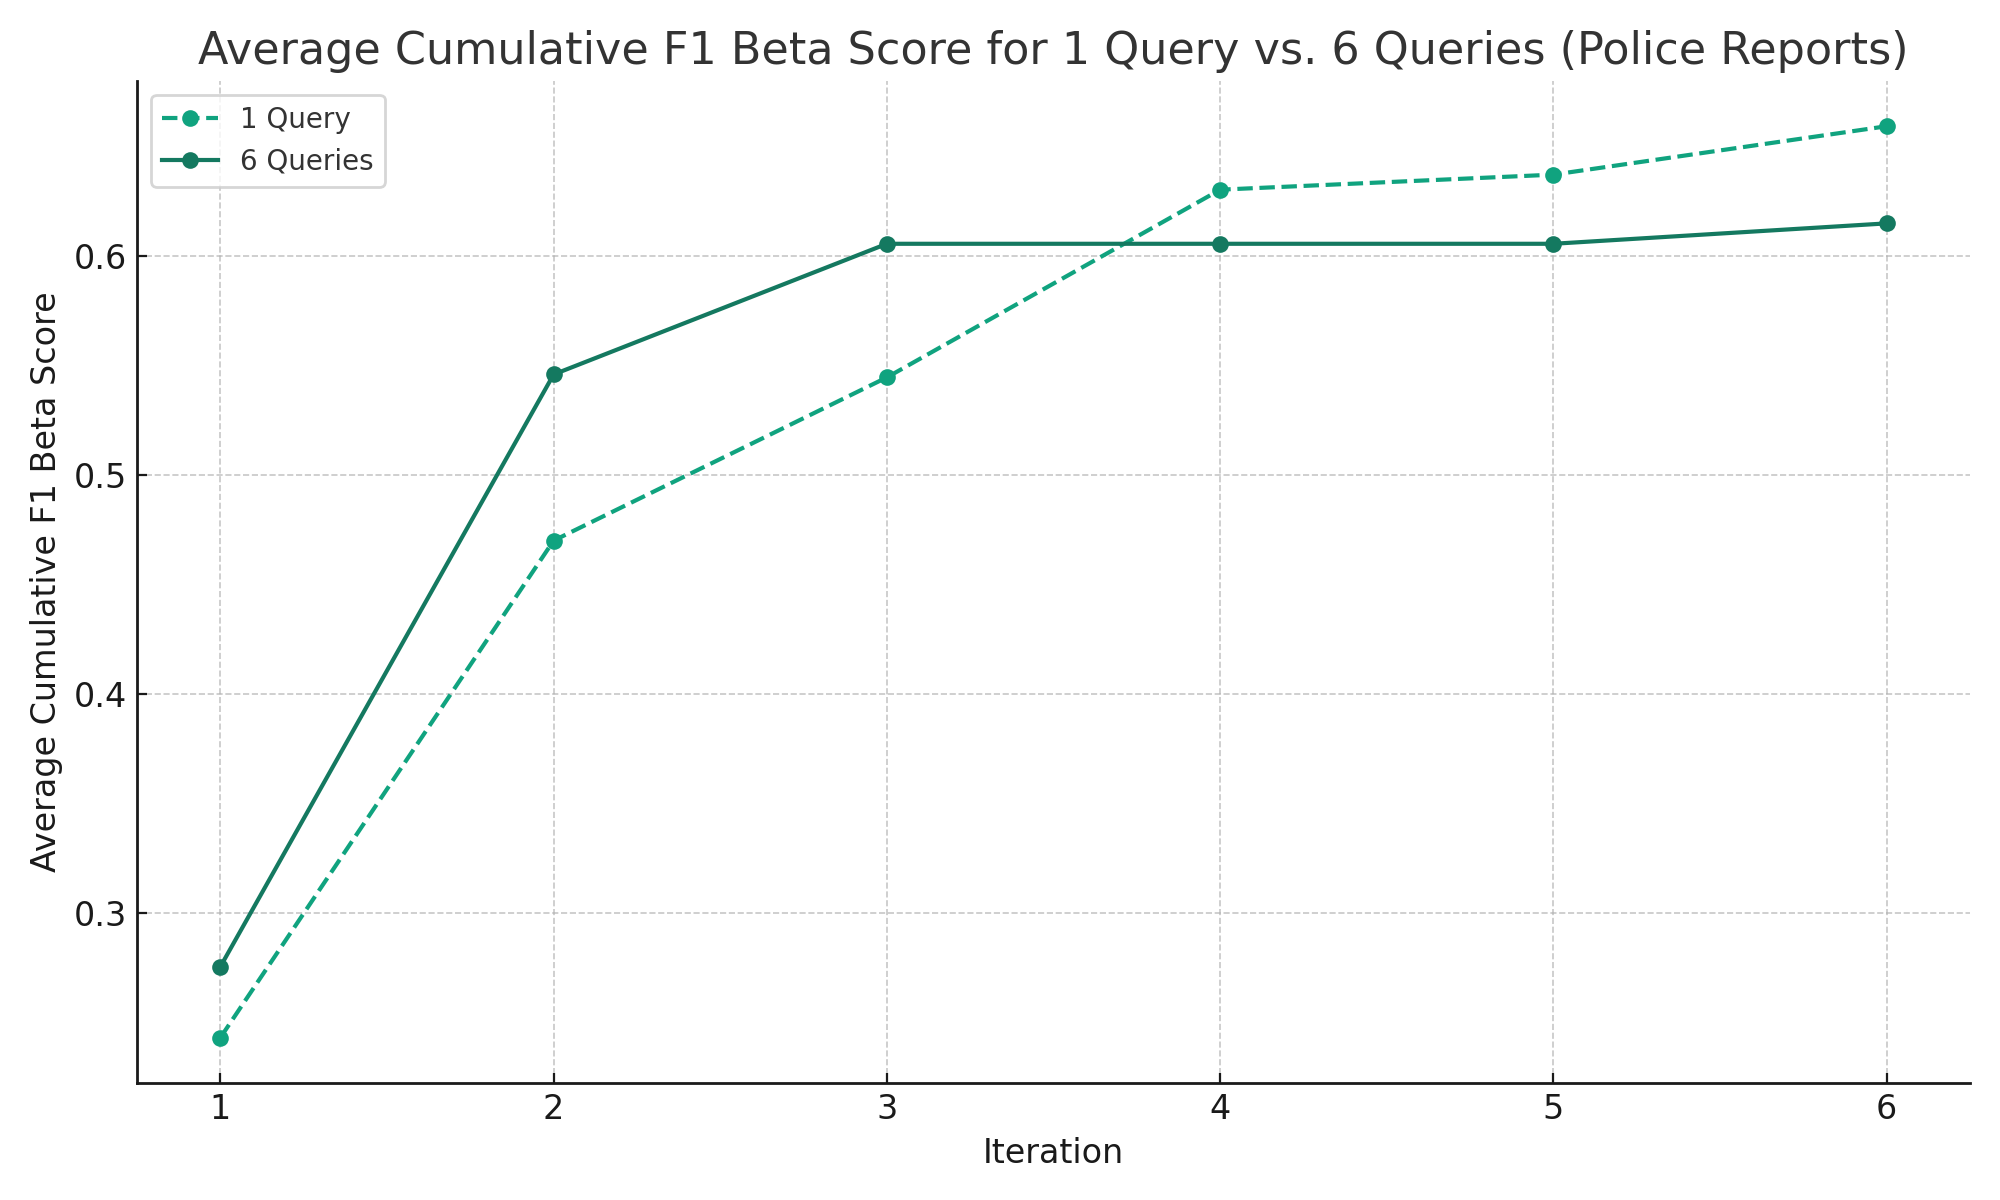
\includegraphics[width=0.8\textwidth]{data/avg_cum_fbeta_police_reports.png}
    \\
    \textit{Figure 1: Average Cumulative F1 Beta Score for 1 Query vs. 6 Queries (Police Reports)}
\end{center}

The analysis of court transcripts, on the other hand, offered a nuanced perspective. Both the singular and the 6 queries methods exhibited an upward trend in their performance metrics up until the 6th iteration.

\begin{center}
    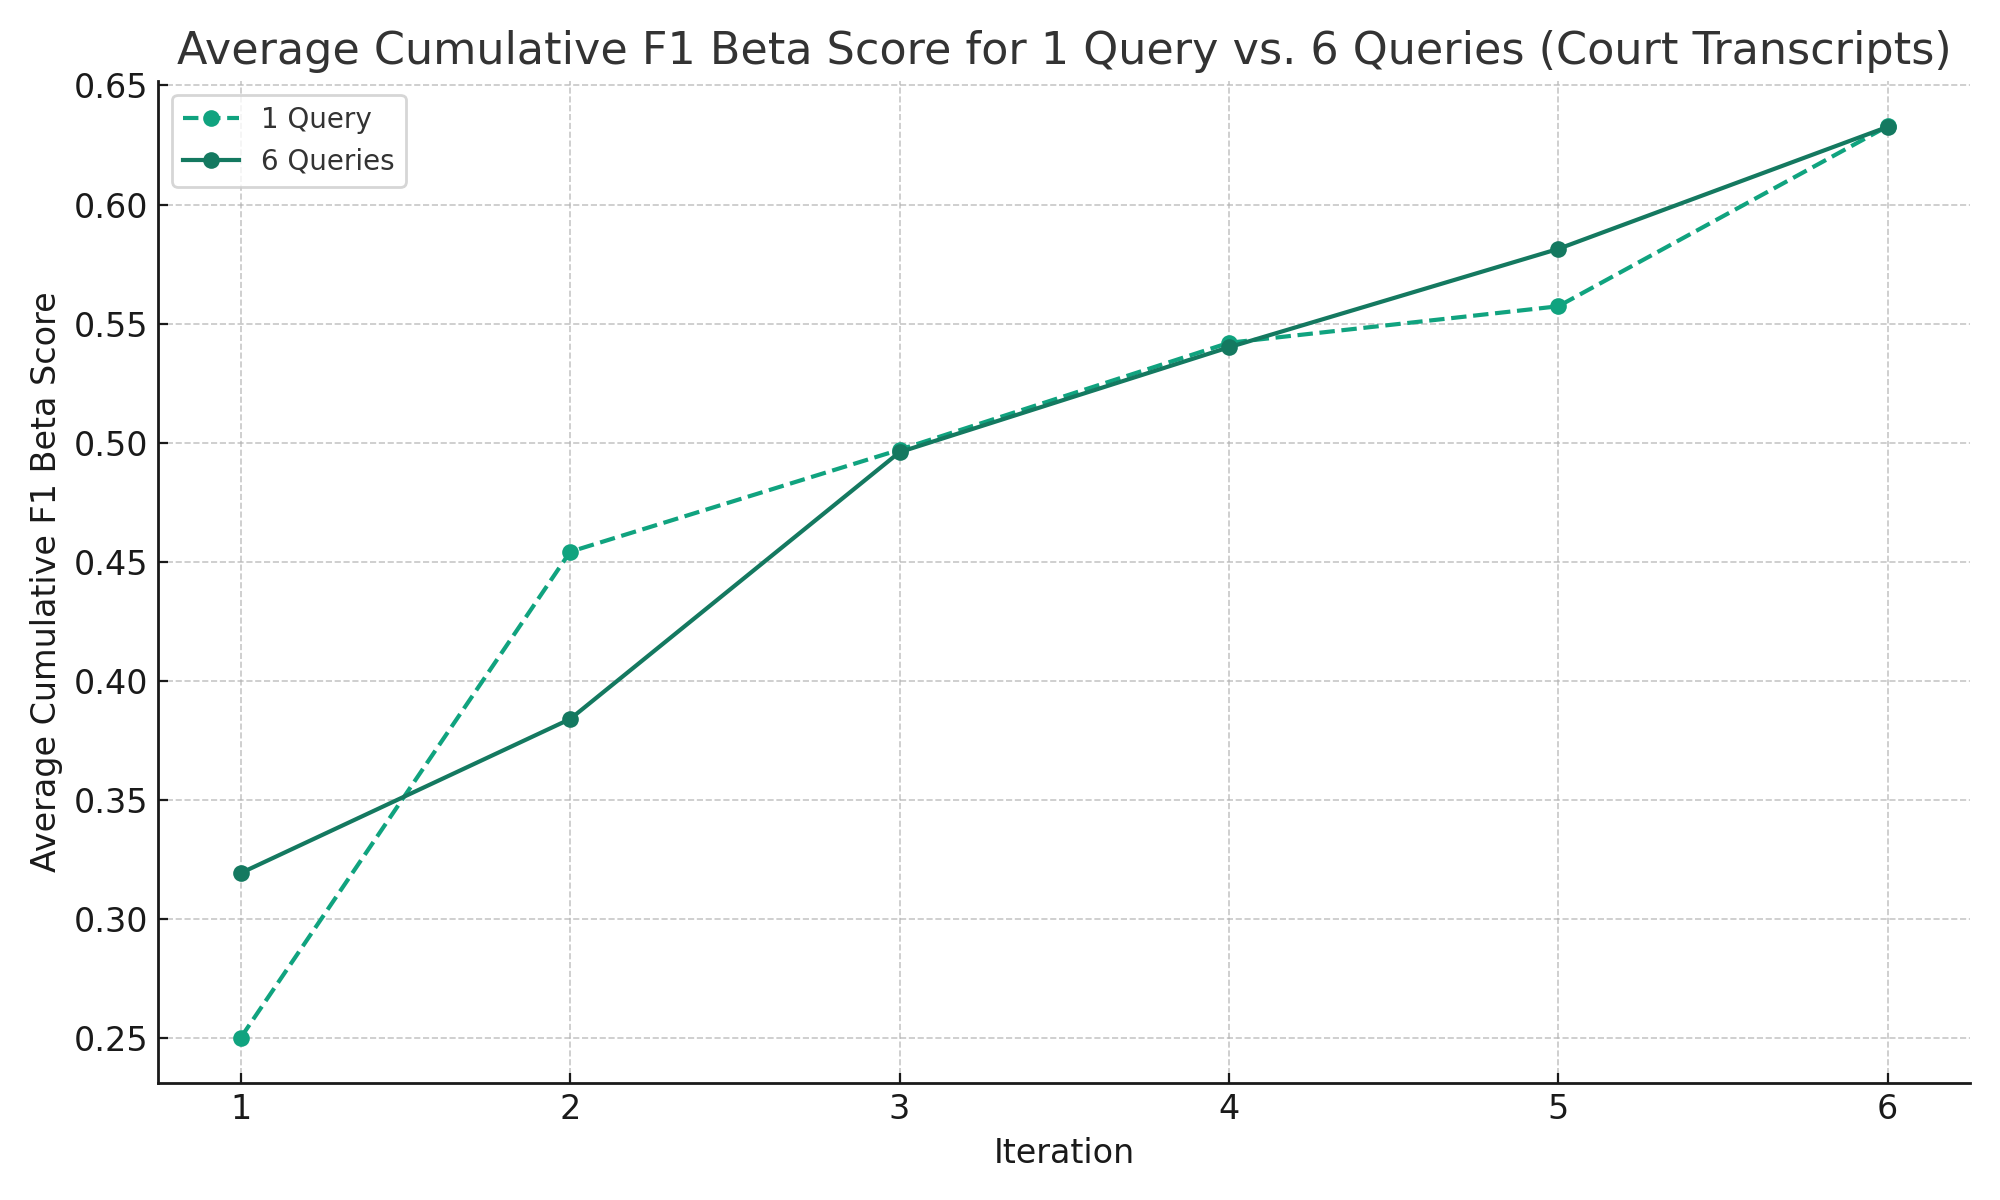
\includegraphics[width=0.8\textwidth]{data/avg_cum_fbeta_court_transcripts.png}
    \\
    \textit{Figure 2: Average Cumulative F1 Beta Score for 1 Query vs. 6 Queries (Transcripts)}
\end{center}

Analyzing the results from both police reports and court transcripts gave us confidence in the singular query method. It consistently demonstrated a balance between performance and computational/cost demands, with diminishing performance gains beyond the 4th iteration in both datasets. Therefore, based on this analysis, the singular query strategy was selected for deployment over 4 iterations for all types of documents. 

\section{Future research/next steps}

Currently, GPT-4's pricing is 0.03 per 1K tokens for inputs and 0.06 per 1K tokens for outputs. In contrast, GPT-3-Turbo-4K is priced at 0.0015 per 1K tokens for inputs and 0.002 per 1K tokens for outputs. This means using GPT-4 is 19x and 29x more expensive, respectively. Given these cost considerations, coupled with challenges our existing GPT-3.5-Turbo-16K model faced in extracting officer details from documents in our FAISS similarity database, we've pivoted our focus towards the GPT-3.5-Turbo-4K model. While the GPT-3.5-Turbo-4K itself isn't new, the capability to fine-tune it was introduced by OpenAI in August 2023, offering a promising avenue for improvement.

In order to address our model's shortcomings, we found ways to efficiently generate additional training data. Using document samples, we extracted details about individual law enforcement officers, their contexts, and roles. Recognizing the potential of GPT-4, we leveraged its capabilities to craft training documents that closely resembled our real-world challenges. We provided GPT-4 with sample documents based on authentic data, enabling it to produce outputs with the stylistic nuances we often encounter---like poor OCR quality, fragmented sentences, inconsistent capitalization, and syntactic inconsistencies.

Here's an example of the training data we generated using GPT-4:

\begin{lstlisting}[breaklines=true]
    { 
        "messages": 
        [{ "role": "system", "content": 
            "As an AI assistant, my role is to meticulously analyze criminal justice documents and extract information about law enforcement personnel. The response will contain: 1) The name of a law enforcement personnel. The individual's name must be prefixed with one of the following titles to be in law enforcement: Detective, Sergeant, Lieutenant, Captain, Deputy, Officer, Patrol Officer, Criminalist, Technician, Coroner, or Dr. Please prefix the name with 'Officer Name:  I will derive this data from the following paragraph: On September 13, DET. X. Y. Allen responded to claims of counterfeit money circulating in the Westside Market. Primary informants were Mrs. Jacobs, a vendor, and Mr. Silva, a customer. FORWARD COPY TO: DETECTIVE DIVISION. INFORMANT DOCS."}, 
            { "role": "user", "content": 'Identify each individual in the transcript, by name, who are directly referred to as officers, sergeants, lieutenants, captains, detectives, homicide officers, and crime lab personnel." }, 
            { "role": "assistant", "content": 
            "Officer Name: DET. X. Y. Allen
            Officer Context: On September 13, DET. X. Y. Allen responded to claims of counterfeit money circulating in the Westside Market. 
            Officer Role: Detective" }] 
    }
    \end{lstlisting}

In our fine-tuning experiments, we worked with four dataset sizes: 25, 50, 75, and 100 examples. Analyzing the outcomes, a clear trend emerged: as we increased the dataset size, the model's performance improved incrementally. Even with the constraints of the 4k token limit, which led us to adjust our K parameter from 25 to 15, our model exhibited differentiated performance across document types. It surpassed the GPT-3.5-Turbo-16k model when processing court transcripts and matched its efficiency for police reports. However, as promising as these strides are, they haven't yet reached the capabilities of GPT-4 (See appendix for GPT-4 results).

\begin{figure}[h]
    \centering
    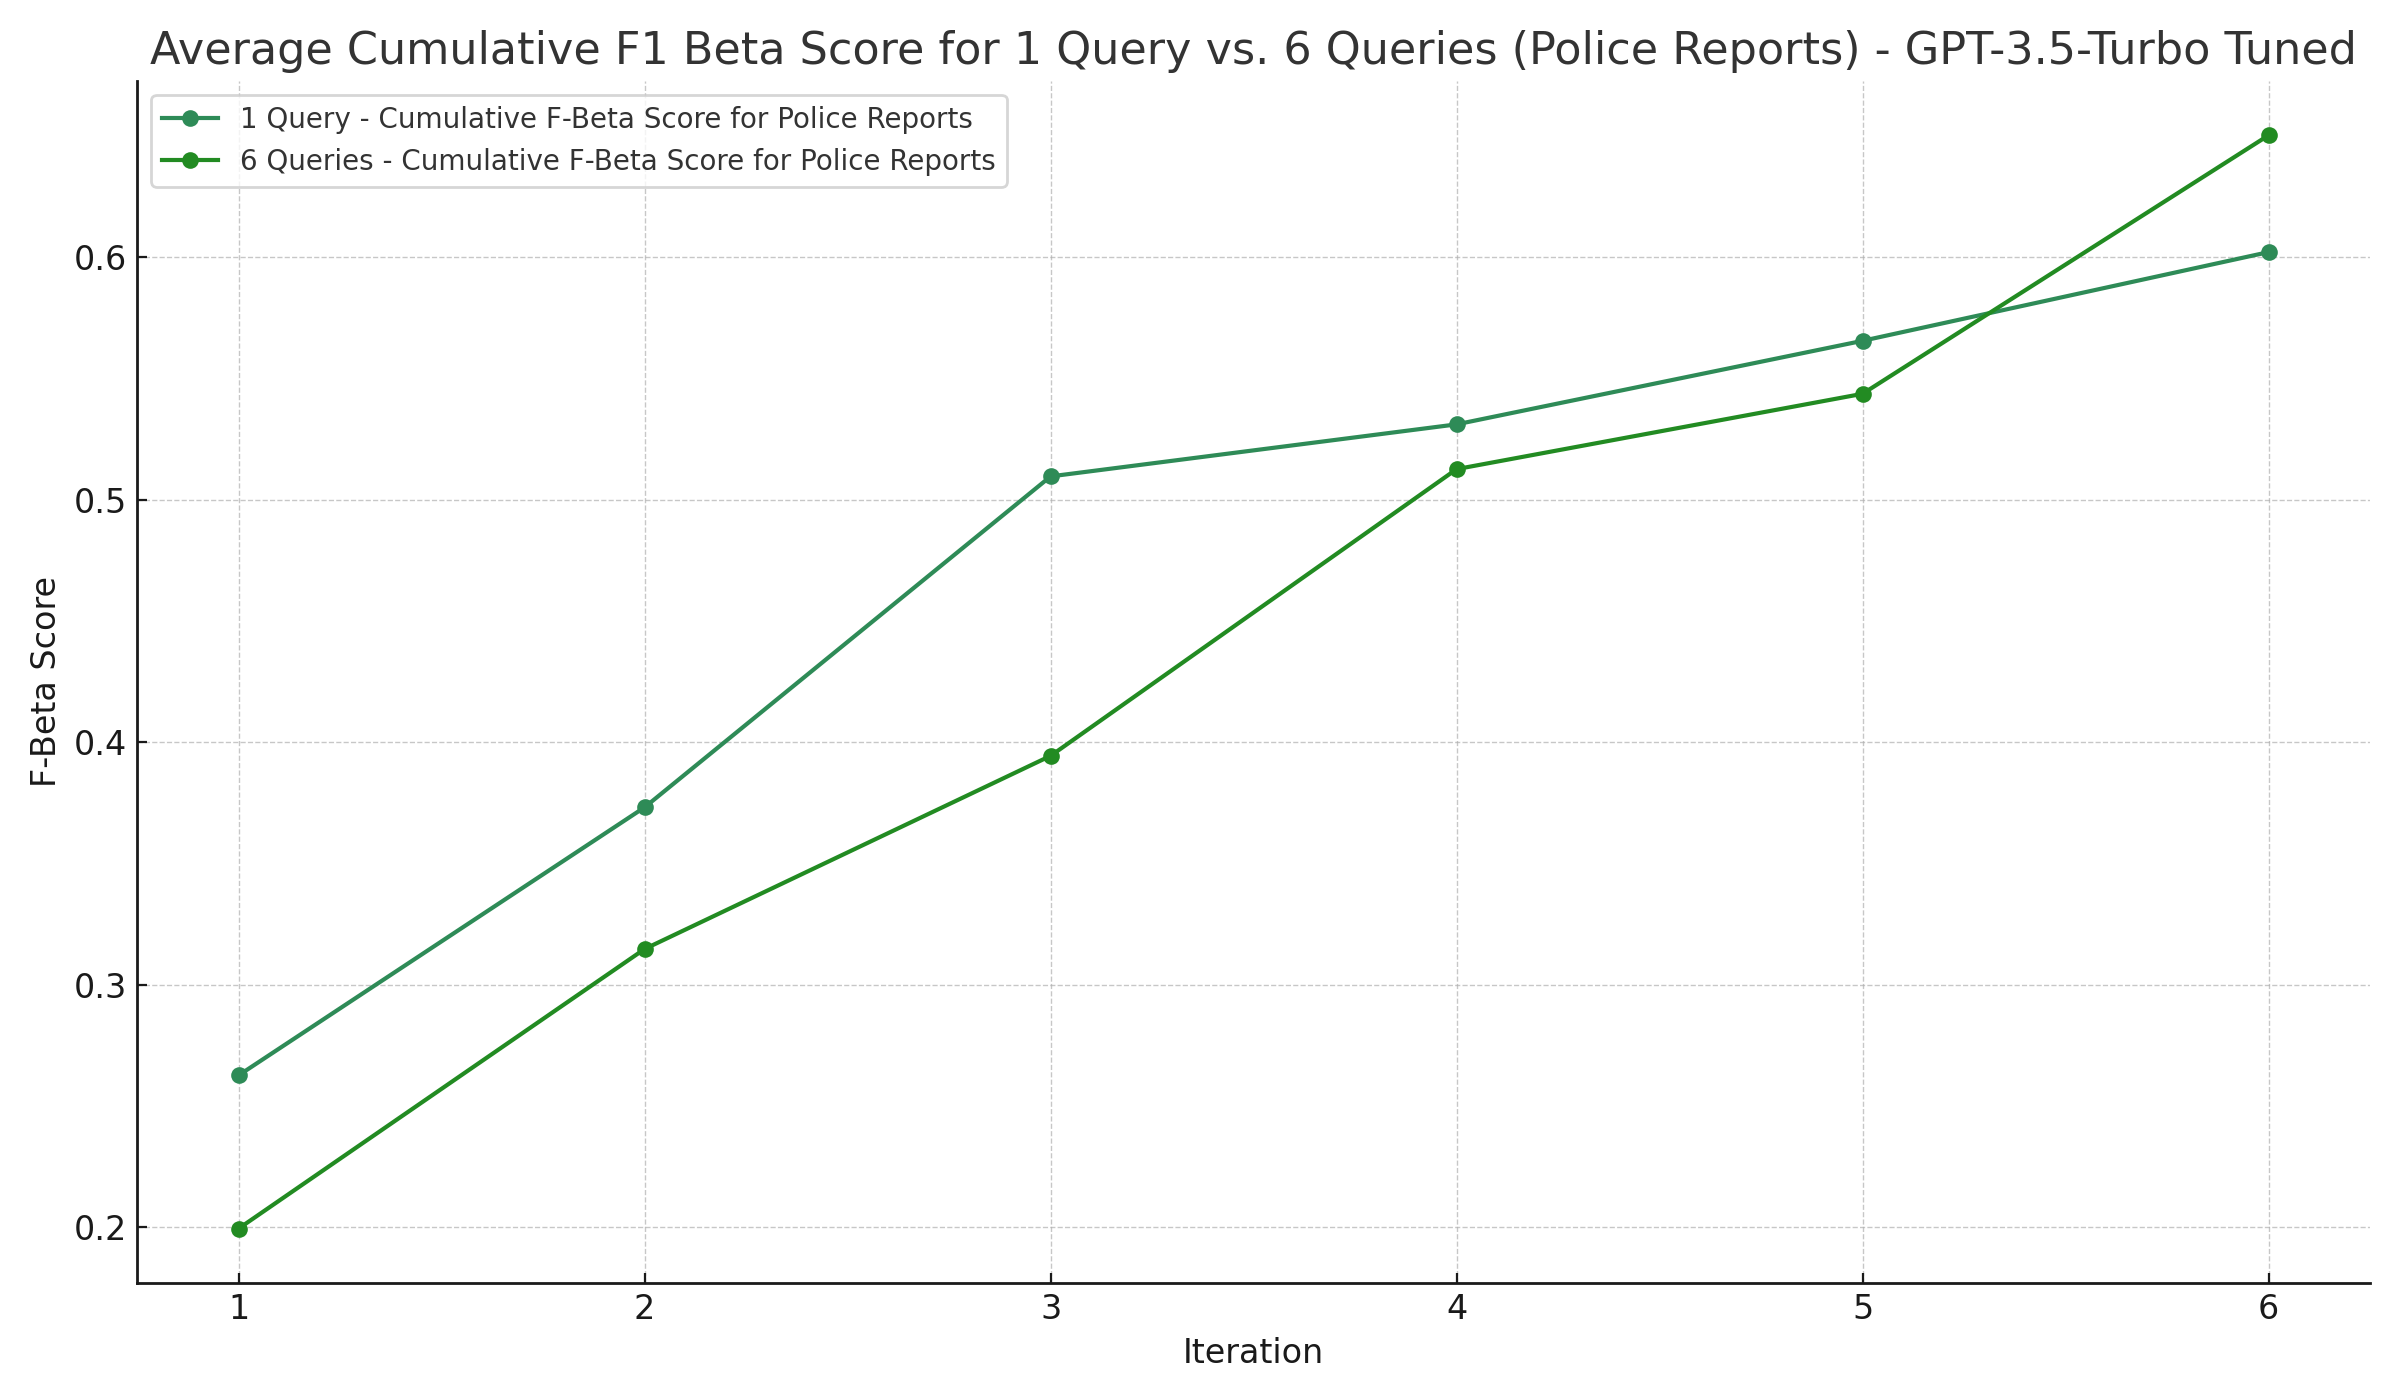
\includegraphics[width=0.7\textwidth]{data/police_reports_graph_tuned.png}
    \caption{Figure 3: Average Cumulative F1 Beta Score for 1 Query vs. 6 Queries (Police Reports) Model: GPT-3}
\end{figure}

\begin{figure}[h]
    \centering
    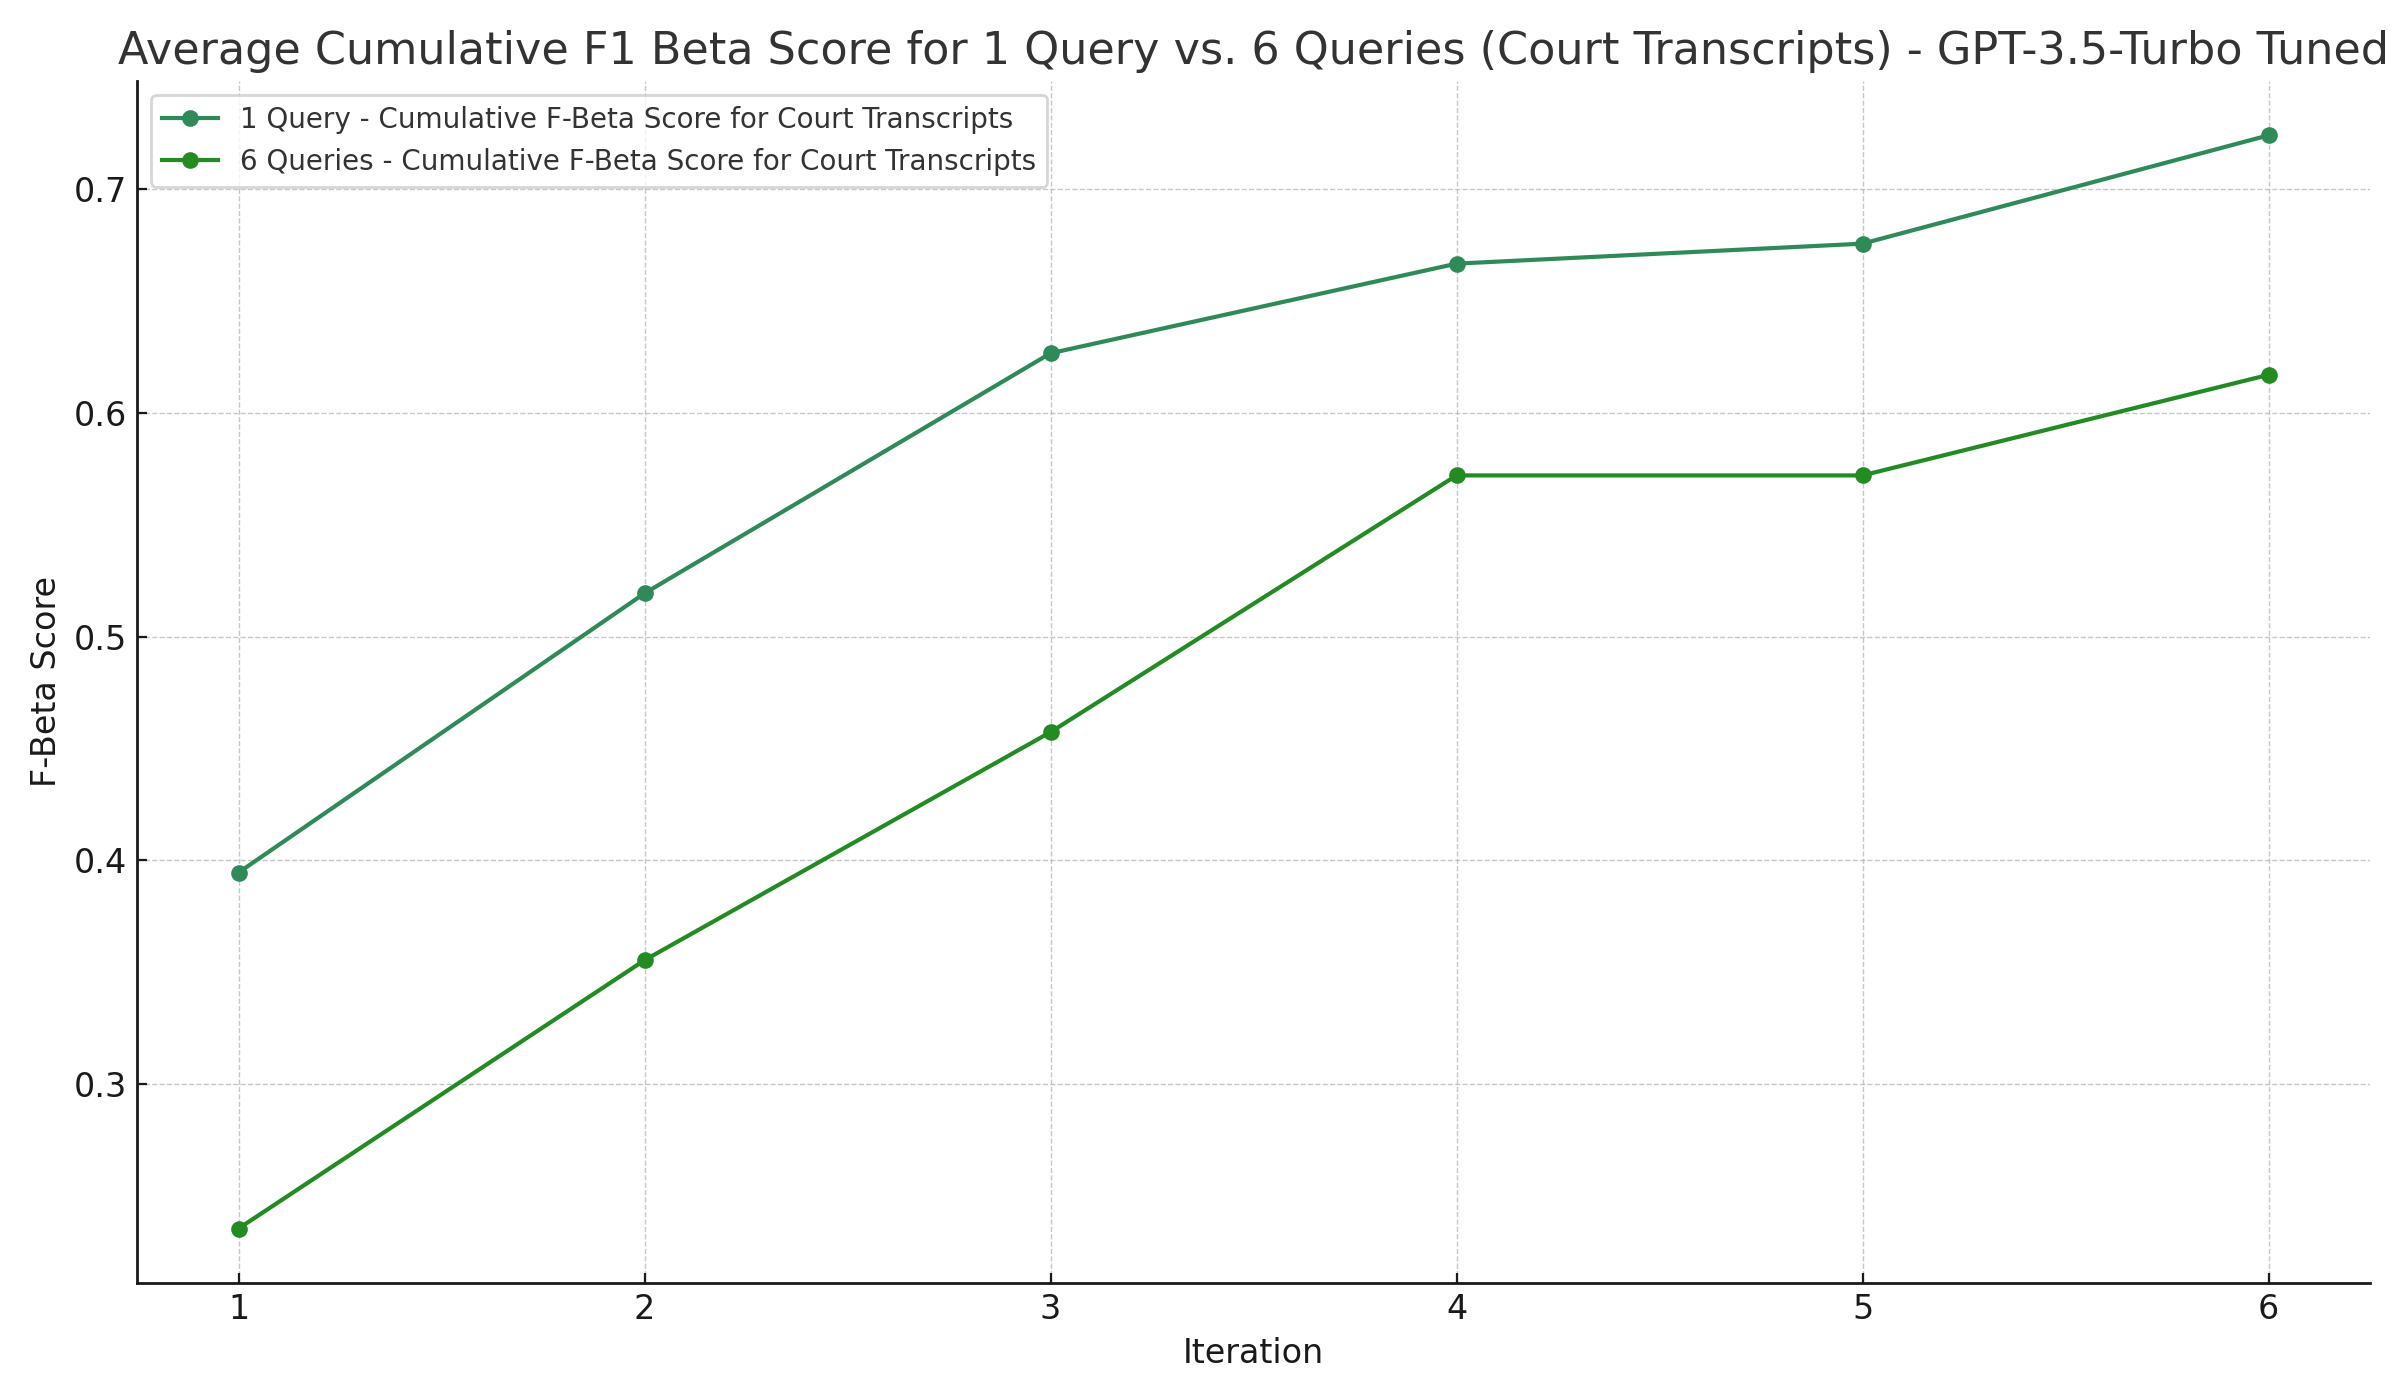
\includegraphics[width=0.7\textwidth]{data/court_transcripts_graph_tuned.png}
    \caption{Figure 4: Average Cumulative F1 Beta Score for 1 Query vs. 6 Queries (Court Transcripts) Model: GPT-3}
\end{figure}

The results from our current fine-tuning experiments with GPT models provide valuable insights into the potential and limitations of AI in data extraction tasks. Our observations underscore the significance of dataset size and quality, as well as the implications of token constraints on model performance. As we move forward:

\begin{itemize}
    \item We will delve deeper into the interplay between token limits and extraction accuracy, particularly in documents with varying complexities.
    \item We'll further investigate the optimal balance between training data volume and model efficiency, exploring potential diminishing returns or inflection points.
    \item Given the differentiated performance across document types, our research will also focus on domain-specific fine-tuning to optimize extraction from court transcripts, police reports, and other legal documents.
\end{itemize}

\section{Appendix}

\begin{itemize}
\item GPT-4 applied to Police Reports

\begin{center}
    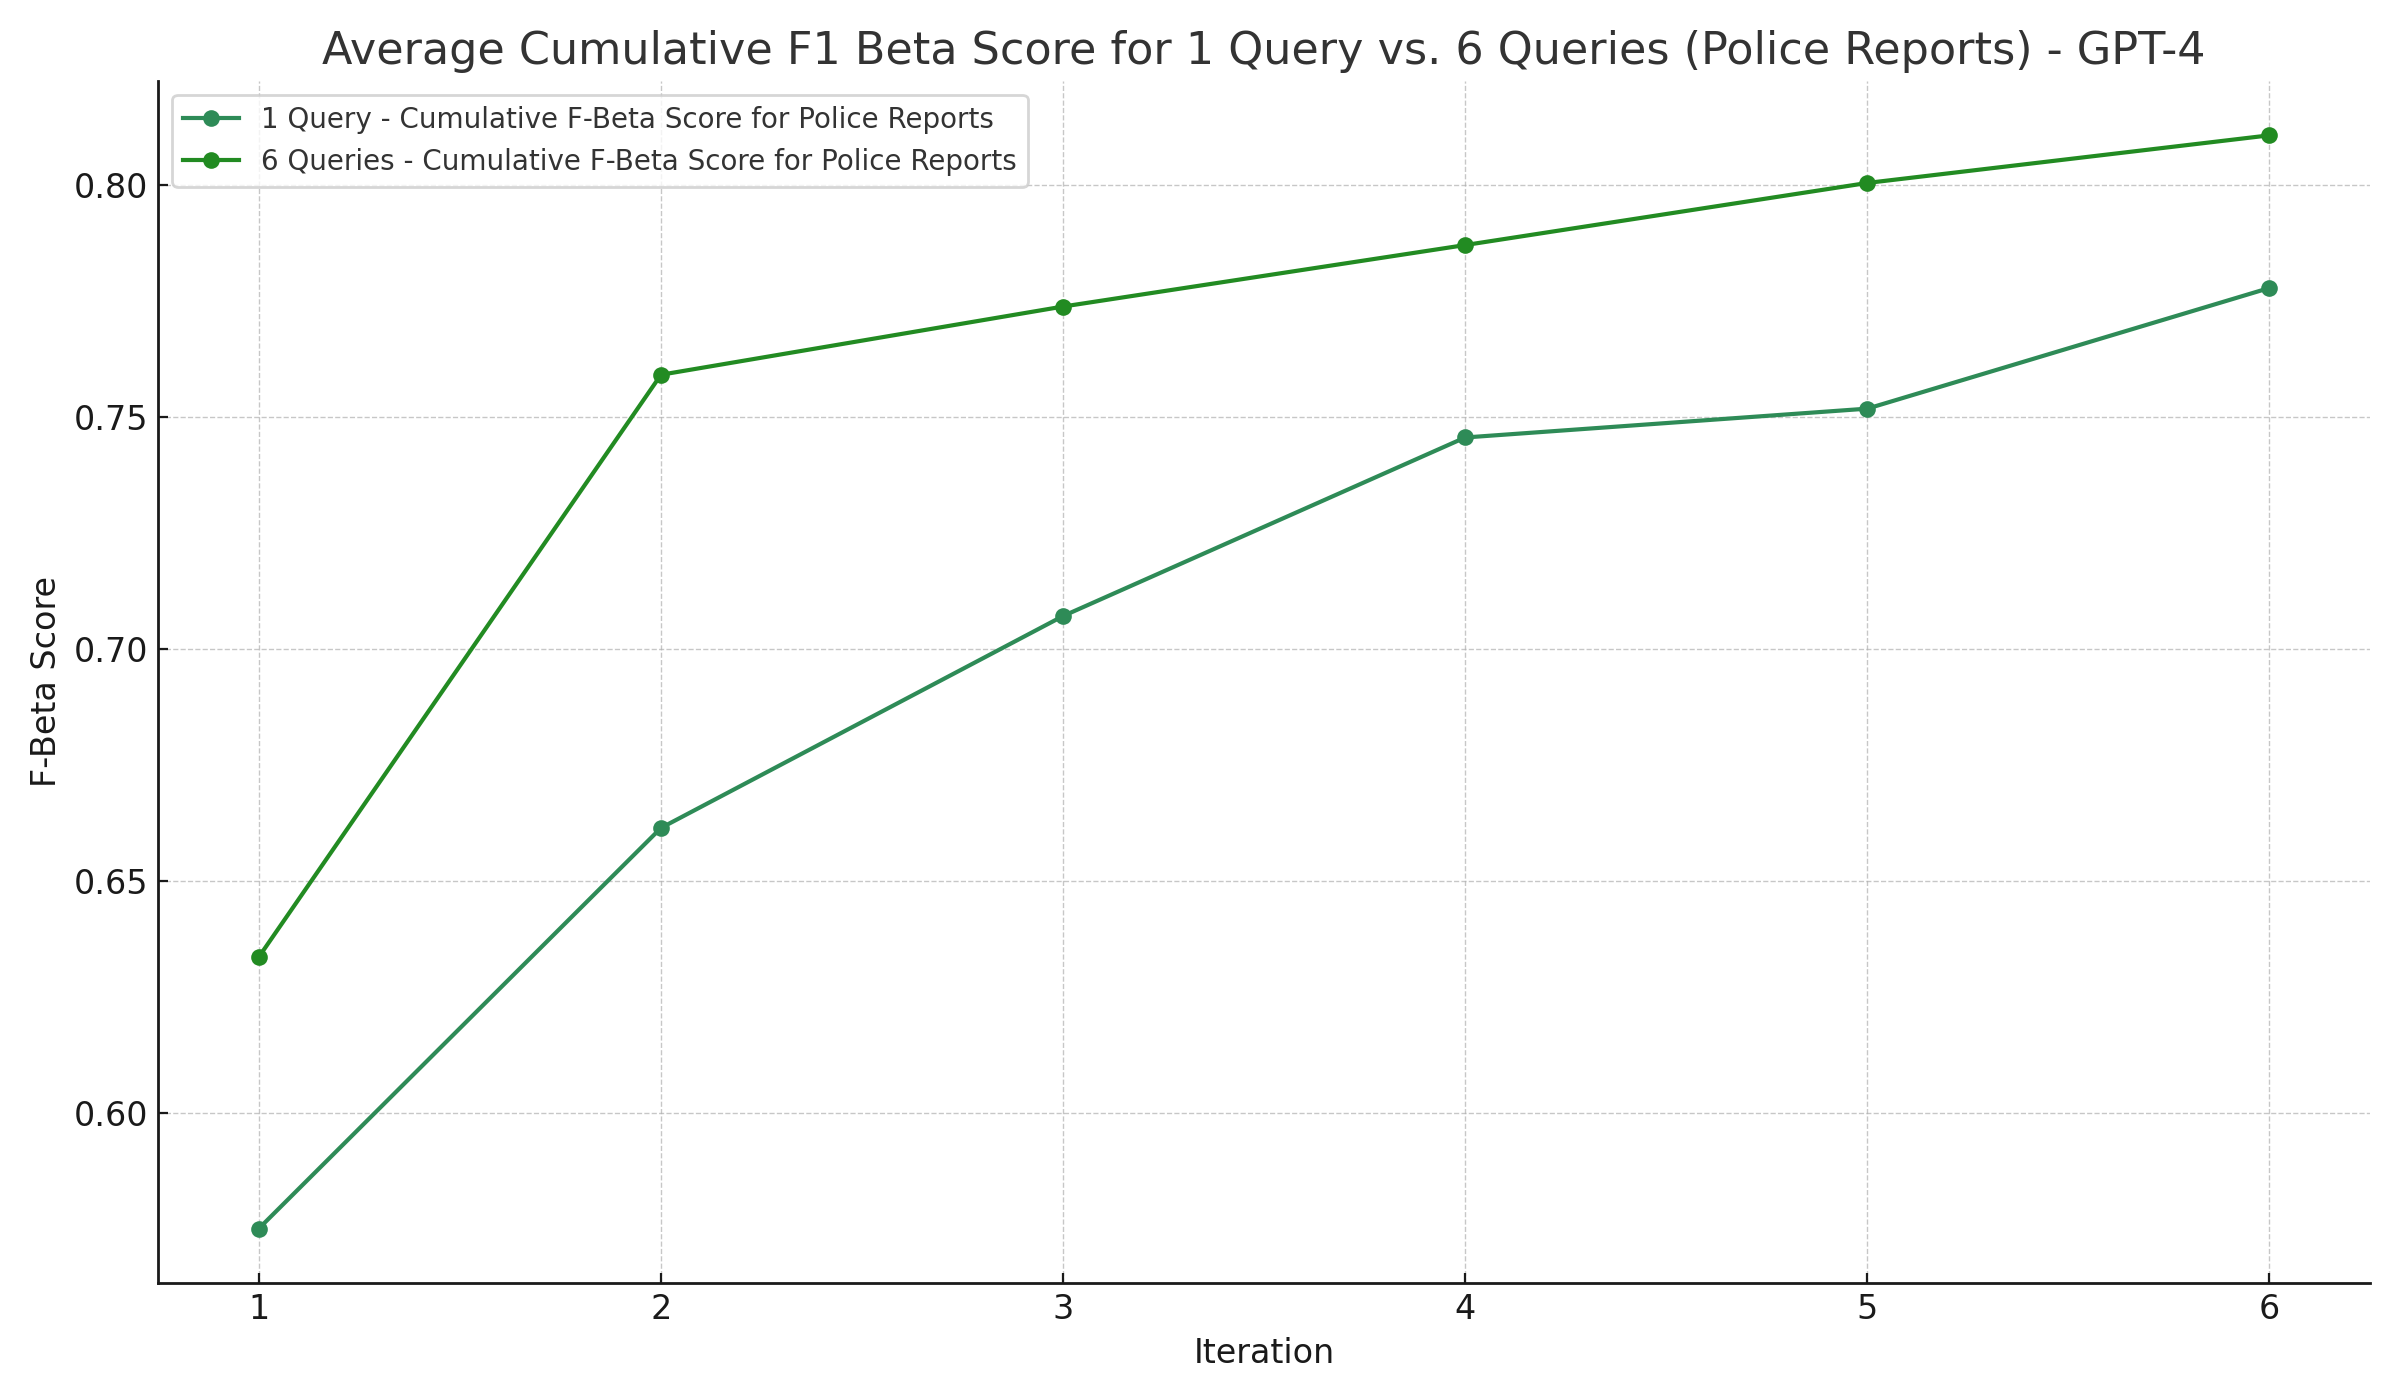
\includegraphics[width=0.6\textwidth]{data/police_reports_graph_gpt-4.png}
    \captionof{figure}{Average Cumulative F1 Beta Score for 1 Query vs. 6 Queries (Police Reports) - Model: GPT-4}
\end{center}

\item GPT-4 applied to Court Transcripts

\begin{center}
    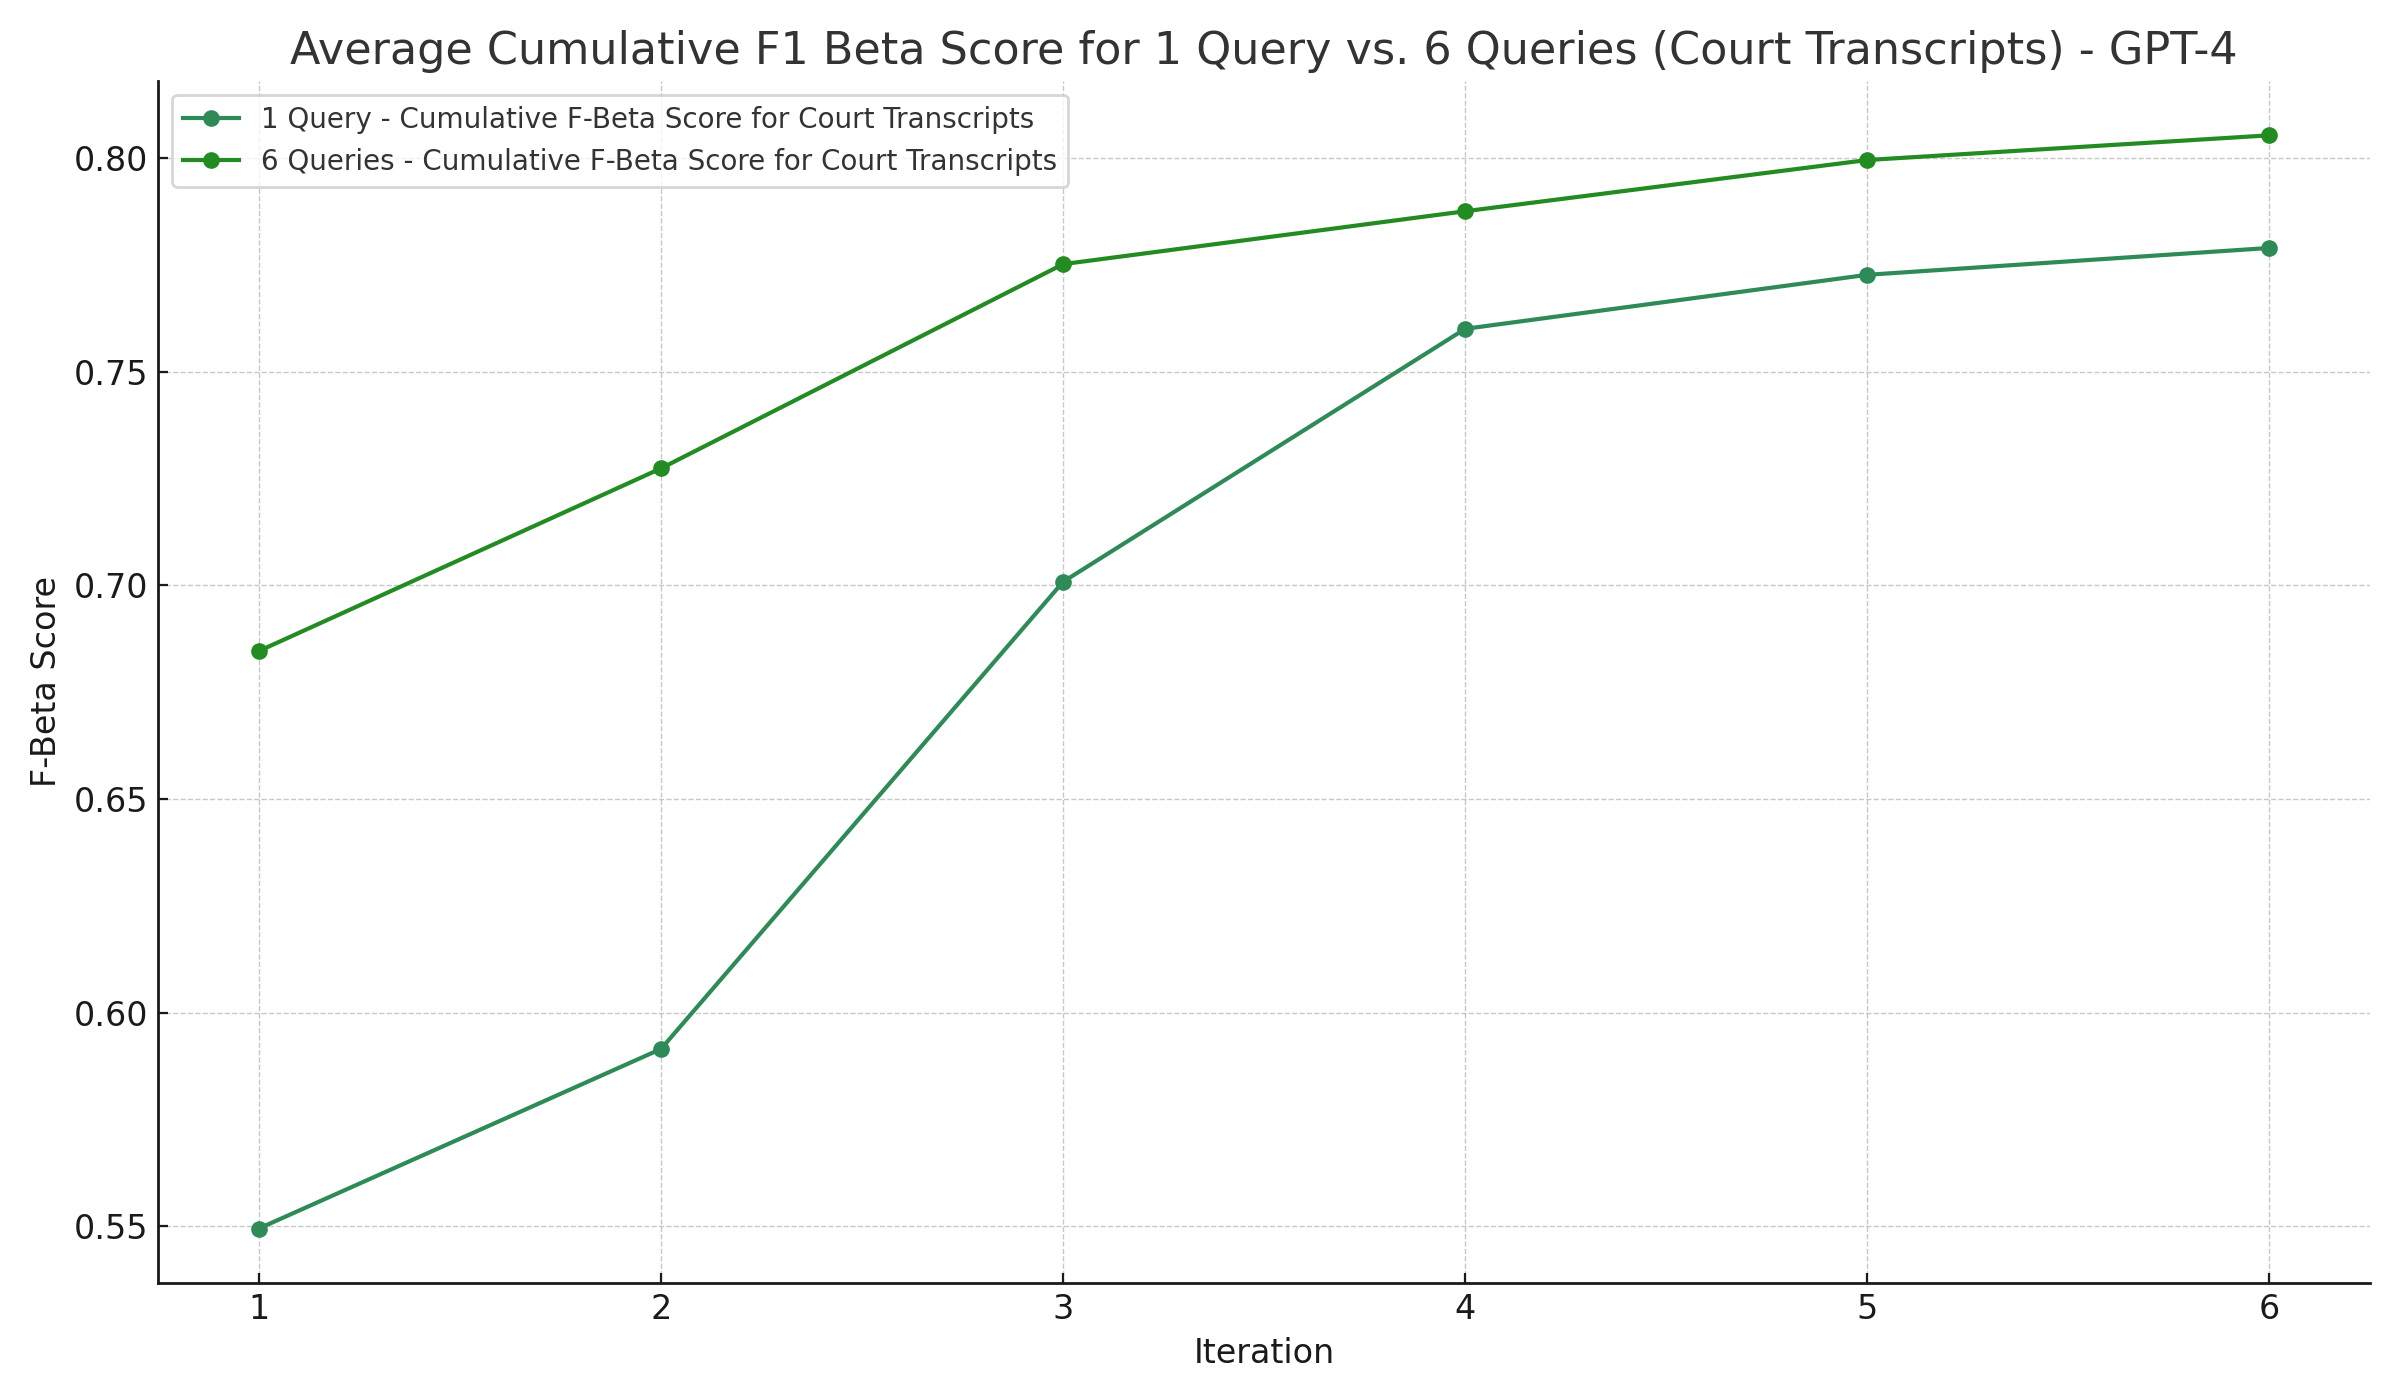
\includegraphics[width=0.6\textwidth]{data/court_transcripts_graph_gpt-4.png}
    \captionof{figure}{Average Cumulative F1 Beta Score for 1 Query vs. 6 Queries (Court Transcripts) - Model: GPT-4}
\end{center}

\end{itemize}

\section*{Acknowledgements}

\begin{itemize}
\item Innocence Project New Orleans: Huy Dao
\item Public Data Works: Rajiv Sinclair, Khoi Pham
\item Human Rights Data Analysis Group: Dr. Megan Price
\item and OpenAI, for their generous donation of research credits, without which we could not have run all of these experiments.
\end{itemize}

\end{document}
